% ============================================================
% f2015tjl_q17_prism.tex —— 2015 天津卷（理科）第 17 题 四棱柱
% ------------------------------------------------------------
% 坐标口径：图内画布 pt，原点 = 源页基准点，x 右正、y 上正。
%   来源：.work/phase3-b11/figure-inventory.md（真实页 pt，原点左上、y 向下）
%   换算：X_tikz = x_page − 236.74 ；  Y_tikz = 329.48 − y_page
% 线宽：全图 0.3985 pt；**虚线节距 2.98883 / 2.98883**（全卷唯一虚线组，清单 §0.4）。
% 实/虚分工：实线 11 条、虚线 7 条（清单 §4.2）。底面四边形 D-C-B-A，A 为被遮挡顶点，
%   故 BC、CD 实线，DA、AB 与对角线 AC 均虚线；一切以 A 为端点的线（AA₁/AB/AC/AD/AB₁/AD₁）
%   皆虚线，与「A 在后」一致。
% N = D₁D 中点 (0.00,81.36)；M = B₁C 中点 (101.01,63.70)，N–M 连线为虚线。
% 照源复刻（清单 §7）：S-7 题设「设 E 为棱 A₁B₁ 上的点」，而**源图未画出 E 点**——不补。
% 要素：18 描边 path（实 11 + 虚 7），填充路径 0；顶点标签 8 + 中点标签 2（清单 §4.4）。
% ============================================================
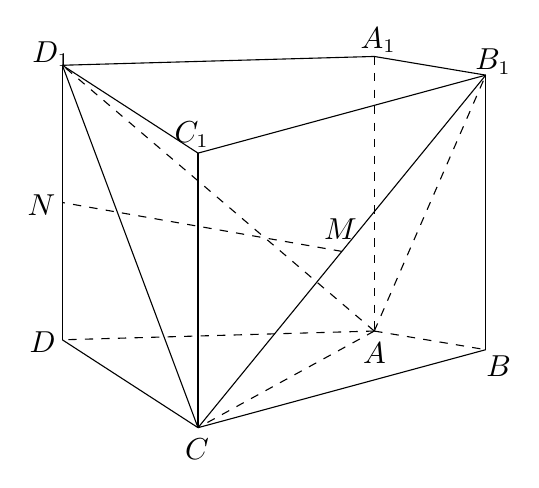
\begin{tikzpicture}[
  x=1pt,y=1pt,                             % 画布单位 = 1 pt（本文件坐标一律为 pt）
  every node/.style={font=\fontsize{10.5pt}{12.6pt}\selectfont,inner sep=0pt},
  s/.style={line width=0.3985pt},
  d/.style={line width=0.3985pt,dash pattern=on 2.98883pt off 2.98883pt},
]

  % ---------- 实线 11 条 ----------
  \draw[s] (0.00,130.96) -- (0.00,31.75);       % 1  D₁D
  \draw[s] (49.02,99.21) -- (49.02,0.00);       % 2  C₁C
  \draw[s] (112.71,134.14) -- (152.99,127.39);  % 3  A₁B₁
  \draw[s] (152.99,127.39) -- (49.02,99.21);    % 4  B₁C₁
  \draw[s] (49.02,99.21) -- (0.00,130.96);      % 5  C₁D₁
  \draw[s] (0.00,130.96) -- (112.71,134.14);    % 6  D₁A₁
  \draw[s] (49.02,0.00) -- (0.00,130.96);       % 7  D₁C
  \draw[s] (49.02,0.00) -- (152.99,127.39);     % 8  B₁C
  \draw[s] (152.99,127.39) -- (152.99,28.18);   % 9  B₁B
  \draw[s] (0.00,31.75) -- (49.02,0.00);        % 10 DC
  \draw[s] (49.02,0.00) -- (152.99,28.18);      % 11 CB

  % ---------- 虚线 7 条 ----------
  \draw[d] (112.71,134.14) -- (112.71,34.92);   % 12 A₁A
  \draw[d] (112.71,34.92) -- (152.99,28.18);    % 13 AB
  \draw[d] (112.71,34.92) -- (49.02,0.00);      % 14 AC
  \draw[d] (112.71,34.92) -- (0.00,31.75);      % 15 AD
  \draw[d] (112.71,34.92) -- (152.99,127.39);   % 16 AB₁
  \draw[d] (112.71,34.92) -- (0.00,130.96);     % 17 AD₁
  \draw[d] (101.01,63.70) -- (0.00,81.36);      % 18 NM（M → N）

  % ---------- 标签（清单 §4.1 / §4.3 实测字形中心）----------
  \node at (-4.04,134.98)  {$D_1$};
  \node at (114.16,139.98) {$A_1$};
  \node at (155.66,132.18) {$B_1$};
  \node at (46.76,105.98)  {$C_1$};
  \node at (-7.14,30.78)   {$D$};
  \node at (112.76,26.98)  {$A$};
  \node at (157.66,22.28)  {$B$};
  \node at (48.66,-7.92)   {$C$};
  \node at (-7.54,80.38)   {$N$};
  \node at (100.46,71.68)  {$M$};

\end{tikzpicture}
